\section{Aufbau}

    \noindent Der Versuch wird mithilfe eines D8-Labordiffraktometer der Firma Bruker-AXS durchgeführt. Dieses ist in \autoref{fig:apparatur}
    zu sehen. Es handelt sich um ein $\Theta$-$\Theta$-Diffraktometer, wobei sich der Detektor und die Röntgenröhre jeweils um den 
    Probentisch bewegen können. 
    \begin{figure}
        \centering
        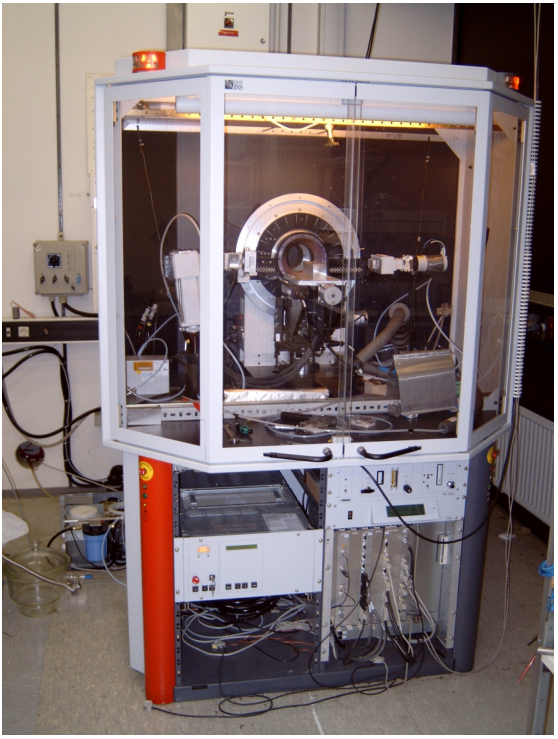
\includegraphics[width=0.4\textwidth]{latex/images/apparatur.png}
        \caption{Das im Versuch benutzte D8-Labordiffraktometer. \cite{katti} }
        \label{fig:apparatur}
    \end{figure}
    Die Röntgenstrahlen werden mithilfe einer Röntgenröhre erzeugt. Diese hat eine Kupferanode und wird mit einem Strom von $\SI{35}{\milli\ampere}$ 
    bei einer Spannung von $\SI{40}{\kilo\volt}$ betrieben. \\
    Das Diffraktometer wird mit dem Programm \enquote{XRD Commander} gesteuert. 

\section{Durchführung}

    \noindent 
    Der Versuch besteht aus der  Justage des Röntgenreflektometers und den anschließenden zwei Messungen.
    Bevor mit der Justage begonnen werden kann, muss der Siliziumwafer mit einer Pinzette vorsichtig möglichst mittig auf den Probentisch gelegt werden. \\
    In der Justage werden alle Scans mit einer Messdauer von $\SI{1}{\second}$ pro Messpunkt durchgeführt.


    \subsection{Justage}

        \noindent Zuerst wird der \textbf{Detektorscan} durchgeführt. Dafür wird der Probentisch aus dem Strahlengang gefahren. Anschließend 
        wird der Detektor im Bereich von $\SI{-0.5}{\milli\metre}$ bis $\SI{0.5}{\milli\metre}$, bei einer Schrittbreite von $\SI{0.02}{\milli\metre} $, bewegt. 
        Damit wird die genaue Nulllage des Detektors ermittelt. Anschließend wird die neue Nulllage auf die Stelle des Intensitätsmaximums 
        dieser Messung gelegt. \\

        \noindent Nach Augenmaß wird der Probentisch an eine gute Position gefahren. Nun wird ein \textbf{Z-Scan} gemacht, wobeider Bereich von 
        $\SI{-1}{\milli\metre}$ bis $\SI{1}{\milli\metre}$, bei einer Schrittweite von $\SI{0.04}{\milli\metre}$, vermessen wird. Hierbei bewegt sich der Probentisch auf der $z$-Achse und fährt 
        sich von unten in den Strahlengang. Sobald die Probe im Strahlengang ist, nimmt die Intensität ab. Es wird anschließend die $z$-Position 
        eingestellt, bei der die halbe Intensität gemessen wurde. \\ 

        \noindent Nun wird ein \textbf{X-Scan} gemacht, wo die Intensität gemessen wird während der Probentisch entlang der $x$-Richtung von 
        $\SI{-20}{\milli\metre}$ bis $\SI{20}{\milli\metre}$ in Schritten von $\SI{1}{\milli\metre}$ durch den Strahlengang geschoben wird. Dabei ergibt sich ein tiefliegendes Plateau, 
        welches dem Durchlaufen der Probe entspricht. Die neue $x$-Koordinate des Probentisch wird auf einen Wert innerhalb des Plateaus gelegt. \\

        \noindent Es wird ein \textbf{Rockingscan} mit einem Winkel $2 \Theta = \num{0}$ durchgeführt. Dabei bewegen sich Röhre und Detektor um die Probe. 
        Es wird von $\SI{-1}{\degree}$ bis $\SI{1}{\degree}$ bei einer Schrittweite von $\SI{0.04}{\degree}$ gemessen. Die Intensitäten sollen
        möglichst einem gleichschenkligen Dreieck entsprechen. Falls dies nicht der Fall ist, wird die $y$-Koordinate des Probentischs verändert. 
        Der Winkel bei dem Intensitätsmaximum wird gespeichert und so werden Röhre und Detektor ausgerichtet. \\

        \noindent Nun liegt die Probe nicht mehr mittig im Strahl und wird mit einem \textbf{zweiten Z-Scan} auf ihre $z$-Koordinate untersucht. 
        Es wird wieder im Bereich von $\SI{-0.5}{\milli\metre}$ bis $\SI{0.5}{\milli\metre}$ in Schritten von $\SI{0.02}{\milli\metre}$ die Intensität gemessen. Die $z$-Koordinate des 
        Probentischs wird auf die Stelle der Hälfte der maximalen Intensität gestellt. \\

        \noindent Um die Probe noch genauer zu justieren wird ein \textbf{zweiter Rockingscan} mit einem Winkel von $2\Theta = \SI{0.3}{\degree}$ 
        durchgeführt. Es wird von $\SI{0}{\degree}$ bis $\SI{0.3}{\degree}$ in Schritten von $\SI{0.005}{\degree}$ gemessen.
        Dabei sollte ein deutlicher Reflex zu sehen sein. 
        Ist dies der Fall, so wird das Maximum des Reflexes durch das Computerprogramm gefunden und diese Auslenkung als Winkel von 
        $\SI{0.15}{\degree}$ gespeichert. \\

        \noindent Aus einem abschließenden \textbf{dritten Z-Scans} kann die halbe Abschattung genauer bestimmt werden. Es wird unter einem Winkel von 
        $2 \Theta = \SI{0.3}{\degree}$ in einem Bereich von $\SI{-0.5}{\milli\metre}$ bis $\SI{0.5}{\milli\metre}$, mit Schritten von $\SI{0.02}{\milli\metre}$,  gemessen. Es wird die $z$-Position 
        gewählt, welche die maximale Intensität aufweist. 

    \subsection{Messung}

        \noindent Nach der Justage des Diffraktometers wird zuerst ein Reflektivitätsscan durchgeführt. Dabei handelt es sich um ein 
        \enquote{Omega/2 Theta} Scan, wobei hier der Winkel zwischen Detektor und Probe genau dem zwischen Probe und Röhre entspricht. 
        Nun werden Röhre und Detektor immer zusammen um die Probe bewegt im Scanbereich von $\SI{0}{\degree}$ bis $\SI{2.5}{\degree}$ bei einer
        Schrittweite von $\SI{0.005}{\degree}$. Die Messzeit pro Messpunkt beträgt hier $\SI{5}{\second}$. \\
        Zusätzlich wird ein diffuser Scan gemacht. Hier ist der Detektorwinkel um $\SI{0.1}{\degree}$ im Bezug zum Röhrenwinkel verschoben. 
        Sonst werden alle Einstellungen beibehalten und die neue Messung gestartet. 
  